\section{Rappel de gestion de base de données relationnelles:}
Au début de l'ère des bases de données, chaque application stockait ses données au sein de sa propre structure unique. Lorsque les développeurs voulaient créer des applications pour utiliser ces données, ils devaient en savoir beaucoup sur la structure spécifique des données afin de trouver les données dont ils avaient besoin. Ces structures de données étaient inefficaces, difficiles à gérer et à optimiser pour obtenir de bonnes performances pour les applications. Le modèle de base de données relationnelle a été conçu pour résoudre le problème que présentent plusieurs structures de données arbitraires.

\subsection{Définition : }
Le modèle relationnel a été introduit pour la première fois par Ted Codd du centre de recherche d’IBM en 1970 dans un papier désormais classique, et attira immédiatement un intérêt considérable en raison de sa simplicité et de ses fondations mathématique.

Dans ce modèle, les données sont représentées par des tables, sans préjuger de la façon dont les informations sont stockées dans la machine. Les tables constituent donc la structure logique du modèle relationnel, d’autre part ces données sont gérées par un système de gestion de bases de données relationnelle (relational database management system, en anglais), qui représente un système intégré pour la gestion unifiée des bases de données relationnelles, il est constitué d’un composant de stockage et d’un composant de gestion de données.

L’interface standard pour une base de données relationnelle est le langage SQL (Structured Query Language) considéré comme le langage de manipulation des données relationnelles le plus utilisé aujourd’hui. Il est devenu un standard de fait pour les SGBD relationnels. Il possède des caractéristiques proches de l’algèbre relationnelle (jointures, opérations ensemblistes) et d’autres proches du calcul des tuples (variables sur les relations). SQL est un langage redondant qui permet souvent d'écrire les requêtes de plusieurs façons différentes.

\begin{figure}[h]
	\centering
    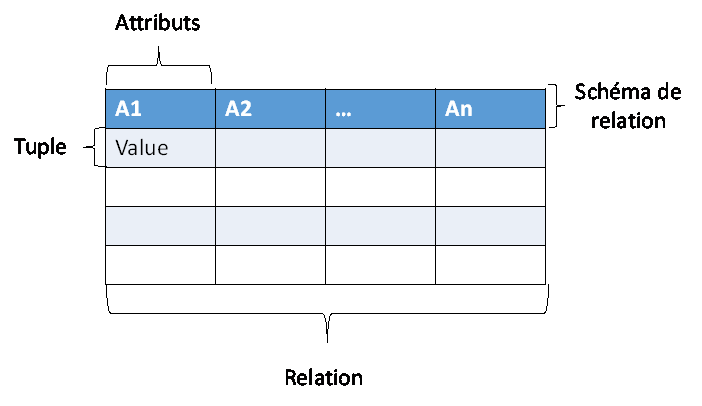
\includegraphics[scale=0.5]{img/part1/4.0.1}
    \caption{Éléments d'une table d'une BDDR.}
\end{figure}
\newpage
\subsection{Les règles CODD :}

Les douze (12) règles de Codd sont un ensemble de règles édictées par Edgar F.Codd afin de définir les caractéristiques que doit présenter un système de gestion de base de données (SGBD) afin d'être considéré comme relationnel (SGBDR). On considère parfois une règle 0, qui stipule que l'intégralité des fonctions du SGBDR doit être accessible par le modèle relationnel.

\begin{enumerate}
\item \textbf{Unicité :} toutes les informations sur les données sont représentées au niveau logique (valeurs dans des colonnes de tables) et non physique.
\item \textbf{Garantie d'accès :} les données sont accessibles sans ambiguïté uniquement par la combinaison du nom de la table, de la clef primaire et du nom de la colonne.
\item \textbf{Traitement des valeurs nulles :} une valeur spéciale doit représenter l'absence de valeur, une information manquante ou une information inapplicable (valeur NULL).
\item \textbf{Catalogue lui-même relationnel :} la description de la base de données doit être accessible comme les données ordinaires (un dictionnaire des données est enregistré dans la base).
\item \textbf{Sous langage de données :} un langage doit permettre de définir les données, définir des vues (visions particulières de la base, enregistrées comme des relations), manipuler les données, définir les contraintes d'intégrité, des autorisations et gérer des transactions.
\item \textbf{Mise à jour des vues :} toutes les vues pouvant théoriquement être mises à jour doivent pouvoir l'être par le système.
\item \textbf{Insertion, mise à jour, et suppression de haut niveau :} le langage doit comporter des ordres effectuant l'insertion, la mise à jour et la suppression de données, aussi bien pour des lots de tuples issues de plusieurs tables que juste pour un tuple unique issu d'une table unique.
\item \textbf{Indépendance physique :} indépendance vis à vis de l'implantation physique des données.
\item \textbf{Indépendance logique :} indépendance vis à vis de l'implantation logique des données (tables, colonnes, etc.).
\item \textbf{Indépendance d'intégrité :} les contraintes d'intégrité doivent pouvoir être définies dans le langage relationnel et enregistrées dans le dictionnaire des données (catalogue).
\item \textbf{Indépendance de distribution :} indépendance de la répartition des données sur divers sites.
\item \textbf{Règle de non subversion :} on ne peut jamais contourner les contraintes (d'intégrité ou de sécurité) imposées par le langage du SGBD en utilisant un langage de programmation de plus bas niveau.
\end{enumerate}

\textit{\textbf{Remarque :} L'ensemble de ces règles indique la voie à suivre pour les systèmes de gestion de bases de données relationnelles. Elles ne sont jamais totalement implémentées, à cause des difficultés techniques que cela représente.}
\newpage
\subsection{Les contraintes des SGBDs relationnels (Propriétés ACID) :}
Selon la théorie des bases de données, les propriétés ACID sont les quatre principaux attributs d'une transaction de données. Il s'agit là d'un des concepts les plus anciens et les plus importants du fonctionnement des bases de données, il spécifie quatre buts à atteindre pour toute transaction. Ces buts sont les suivants :

\begin{enumerate}
\item \textbf{Atomicity (Atomicité) :} Lorsqu’une transaction est effectuée, toutes les opérations qu’elle comporte doivent être menées à bien : en effet, en cas d’échec d’une seule des opérations, toutes les opérations précédentes doivent être complètement annulées, peu importe le nombre d’opérations déjà réussies. En résumé, une transaction doit s’effectuer complètement ou pas du tout.

\textit{\textbf{Exemple:} une transaction qui comporte 3000 lignes qui doivent être modifiées, si la modification d’une seule des lignes échoue, alors la transaction entière est annulée. L’annulation de la transaction est toute à fait normale, car chaque ligne ayant été modifiée peut dépendre du contexte de modification d’une autre, et toute rupture de ce contexte pourrait engendrer une incohérence des données de la base.}

\item \textbf{Consistancy (Cohérence) :} Avant et après l’exécution d’une transaction, les données d’une base doivent toujours être dans un état cohérent. Si le contenu final d’une base de données contient des incohérences, cela entraînera l’échec et l’annulation de toutes les opérations de la dernière transaction. Le système revient au dernier état cohérent. La cohérence est établie par les règles fonctionnelles.

\textit{\textbf{Exemple :} Un système doit être capable de reconnaître qu'une facture est liée à un client et aux éléments factures. Il doit être capable d'éviter, par exemple, la suppression d'un client s'il existe encore des factures pour ce client, et la suppression d'une facture qui a des éléments associées.}

\item \textbf{Isolation (Isolation) :} La caractéristique d’isolation permet à une transaction de s’exécuter en un mode isolé. En mode isolé, seule la transaction peut voir les données qu’elle est en train de modifier, c’est le système qui garantit aux autres transactions exécutées en parallèle une visibilité sur les données antérieures. Ce fonctionnement est obtenu grâce aux verrous système posés par le SGBD. 

\textit{\textbf{Exemple :} Prenons l’exemple de deux transactions A et B : lorsque celles-ci s’exécutent en même temps, les modifications effectuées par A ne sont ni visibles, ni modifiables par B tant que la transaction A n’est pas terminée et validée.}

\item \textbf{Durability (Durabilité) :} Toutes les transactions sont lancées de manière définitive. Une base de données ne doit pas afficher le succès d’une transaction pour ensuite remettre les données modifiées dans leur état initial. Pour ce faire, toute transaction est sauvegardée dans un fichier journal afin que, dans le cas où un problème survient empêchant sa validation complète, elle puisse être correctement terminée lors de la disponibilité du système.
\end{enumerate}
\newpage
\subsection{Limite des bases de données relationnelles :}
Les bases de données existent maintenant depuis environ 56 ans et le modèle relationnel depuis environ 46 ans, pendant plusieurs décennies, ce modèle bien très puissant, représentait la solution parfaite pour les différents acteurs dans le domaine de gestion des données, néanmoins ces architectures ont atteints leurs limites pour certains services ou sites manipulant de grandes masses de données, tels que Google, Facebook, etc. En effet ce genre de sites possède plusieurs millions voire des milliards d’entrées dans leurs bases de données et tout autant de visites journalières, en conséquence les données sont distribuées sur plusieurs machines, de plus pour des raisons de fiabilité ces bases de données sont dupliquées pour que le service ne soit pas interrompu en cas de panne.

Malheureusement le modèle relationnel présente quelques problèmes liés à ce passage à l’échelle tel que :

\subsubsection{1. Problème lié à l’application des propriétés ACID en milieu distribué :}
Une base de données relationnelle est construite en respectant les propriétés ACID (Atomicité, Cohérence, Isolation, Durabilité), ses propriétés bien que nécessaires à la logique du relationnel nuisent fortement aux performances et en particulier la propriété de cohérence.

En effet, la cohérence est très difficile à mettre en place dans le cadre de plusieurs serveurs (environnement distribué), car pour que celle-ci soit respectée tous les serveurs doivent être des miroirs les uns des autres, de ce fait deux problèmes apparaissent :
\begin{itemize}[label=\textbullet]
\item Le coût en stockage est énorme car chaque donnée est présente sur chaque serveur.
\item Le coût d’insertion/modification/suppression est très grand, car on ne peut valider une transaction que si on est certain qu’elle a été effectuée sur tous les serveurs et le système fait patienter l’utilisateur durant ce temps.
\end{itemize}

\begin{figure}[h]
	\centering
    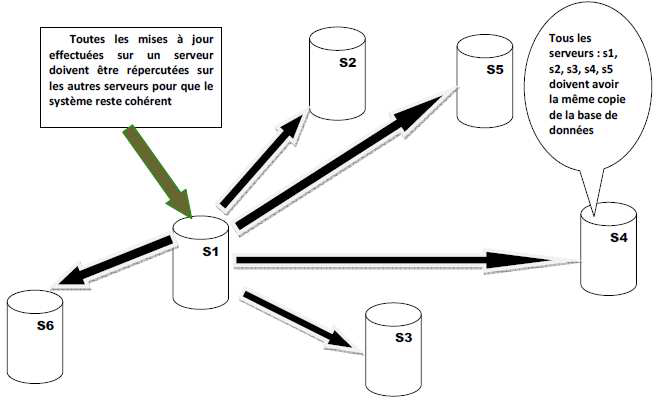
\includegraphics[scale=0.5]{img/4.0.2}
    \caption{Problème lié aux propriétés ACID en milieu distribué}
\end{figure}

\subsubsection{2. Pas de schéma de base de données hiérarchique :  }
Contrairement aux bases de données orientées objet, les bases de données relationnelles n'offrent pas la possibilité d'implémenter des schémas de base de données avec des classes hiérarchiquement structurées. Des concepts tels que les entités subordonnées qui héritent de propriétés d'entités supérieures ne peuvent pas être implémentés avec elles. Par exemple, on ne peut pas créer de sous-tuples avec eux. Tous les tuples d'une base de données relationnelle se trouvent au même niveau hiérarchique.

\subsubsection{3. Problème de requête non optimale dû à l’utilisation des jointures :}
Imaginons une table contenant toutes les personnes ayant un compte sur Facebook, soit 1.55 milliards d’utilisateurs actifs par mois les données dans une base de données relationnelle classique sont stockées par lignes, ainsi si on effectue une requête pour extraire tous les amis d’un utilisateur donné, il faudra effectuer la jointure entre la table des usagers et celle des amities (chaque usagr ayant au moins un ami) puis parcourir le produit cartésien de ces deux tables. De ce fait, on perd énormément en performances en raison du temps consommé pour stocker et parcourir une telle quantité de données.

\subsubsection{4. Problème lié à la gestion des objets hétérogènes: }

« Le stockage distribué n’est pas la seule contrainte qui pèse à ce jour sur les systèmes relationnels» disait Carl STROZZI. Au fur et à mesure du temps, les structures de données manipulées par les systèmes sont devenues de plus en plus complexes en contrepartie les moteurs de stockage évoluant peu. Le principal point faible des modèles relationnels est l’absence de gestion d’objets hétérogènes ainsi que le besoin de déclarer au préalable l’ensemble des champs représentant un objet.

D’autre part le modèle relationnel est fondé sur un modèle mathématique solide s’appuyant sur des concepts simples qui font sa force en même temps que sa faiblesse.

Nous expliquerons quelques limites :

\begin{enumerate}
\item \textbf{Surcharge sémantique :} Le modèle relationnel s’appuie sur un seul concept (la relation) pour modéliser à la fois les entités et les associations entre ces entités. Il existe donc un décalage entre la réalité et sa représentation abstraite.
\item \textbf{Types de données :} Ces modèles sont limités à des types simples (entiers, réels, chaînes de caractères), les seuls types étendus se limitant à l’expression de dates ou de données financières, ainsi que des conteneurs binaires de grande dimension (BLOB, pour Binary Large OBjects) qui permettent de stocker des images ainsi que des fichiers audio ou vidéos. Ces BLOBs ne sont toutefois pas suffisants pour représenter des données complexes (pas de structure), les mécanismes de contrôle BD sont inexistants, et le langage de requêtes (SQL) ne possède pas les opérateurs correspondant aux objets stockés dans ces BLOBs.
\end{enumerate}

\subsubsection{5. Le partitionnement de données:}
L’un des problèmes de la normalisation dans un SGBDR concerne la distribution des données et du traitement. S’il y a des données stockées ayant un rapport entre elles, comme des clients, des commandes, des factures, des lignes de facture, etc., dans des tables différentes, des problèmes surgiront en cas de partitionnement de ces données. Pour y remédier, il faut alors s’assurer que les données en rapport les unes avec les autres se trouvent sur le même serveur.




\newpage
\subsection{Exemples de bases de données relationnelles}
Les systèmes de gestion de bases de données relationnelles (SGBDR) les plus couramment utilisés sont donnés comme suit :

\begin{itemize}[label=\textbullet]
\item \textbf{Db2 :} Est l'un des SGBD relationnelles propriétaire d'IBM 3 disponible aux utilisateurs sous licence commerciale.
\item \textbf{Microsoft SQL Server :} Le système de gestion de base de données de Microsoft 4 en langage SQL est disponible sous une licence par utilisateur payante.
\item \textbf{MySQL :} Est le SGBDR open source 5 le plus utilisé dans le monde. Depuis son acquisition par Oracle, MySQL est commercialisé sous une double licence. La communauté des développeurs d'origine poursuit le projet sous le nom de MariaDB.
\item \textbf{PostgreSQL :} avec PostgreSQL, les utilisateurs peuvent accéder gratuitement à un système de gestion de base de données relationnel-objet (SGBDRO). Le développement ultérieur est effectué par une communauté open source.
\item \textbf{Oracle Database :} le système de gestion de base de données relationnelle de la société du même nom Oracle 6 est commercialisé sous licence propriétaire contre rémunération.
\item \textbf{SQLite :} est une bibliothèque appartenant au domaine public contenant un système de gestion de bases de données relationnelles.
\end{itemize}

\textbf{Résumé :} Le schéma relationnel des bases de données est clair, mathématiquement solide et a fait ses preuves dans la pratique depuis plus de 40 ans. Pourtant, le stockage des données dans des tables structurées ne répond pas à toutes les exigences des technologies modernes de l'information.
\newpage